\section{A New Construct and A New Model}
\note{Timing: \unit[\about35]{min}}{
Purpose:
\begin{itemize}
\item Introduction to the spring potential energy system and the simple oscillator model.  
\end{itemize}
This is an introduction to the spring potential energy system and the simple oscillator model.  Students should know that the indicator that indicates change in this system is the distance from the equilibrium position (compressed or stretched).  They should be able to model oscillation using the energy-interaction model.  They also should have some sense of the fact that the "stretchiness" of the spring would affect the potential energy change, but they do not need to know the algebraic details, yet. 

Learning Outcomes:
\begin{itemize}
\item Understand that a simple oscillator has a potential energy ($PE_{spring-mass}$ or $PE_{m-s}$). 
\item Understand and know that the indicator for the PE is the distance of the mass from its equilibrium position, either compressed or stretched.
\item Be able to model the oscillation of a mass-spring system using the Energy-Interaction Model.
\end{itemize}
}

\label{act2.1.2}

\begin{overview}
\textbf{Overview:} A third mechanical energy system -- in addition to \emph{translational kinetic} energy $KE_\text{translational}$ and \emph{gravitational potential} energy $PE_\text{gravity}$ -- is the \emph{spring-mass} energy $PE_\text{spring-mass}$, introduced here in the context of the \SOModel{}.
\end{overview}

\subsection{Oscillating Spring-Mass}
\label{oscspringmass}
Many physical systems oscillate. The spring-mass system that you are going to examine is one example of many such systems that can be modeled using the \SOModel{}.
\note{Notes on \ref{oscspringmass}
:}{
\begin{itemize}
\item Suggest to students to position the pointer so that it points at the center of 200 g mass.
\item Students sometimes have a hard time with the fact that the maximum speed occurs as the mass passes through the equilibrium position, which was defined as the place where it was originally at rest.  They also may have trouble with the fact that when the mass changes direction (at the top and bottom) its speed is zero.  Sometimes referring to a swing set helps them to see the motion better.

The spring-mass system is �symmetric�, but a greater initial displacement certainly results in a more vigorous motion. Try this: hide the spring-mass from the students (use a piece of paper) and start it going.  Then reveal it and ask if you started from above or below equilibrium.

\item The two systems involved are the spring-mass potential energy system (indicator is distance from equilibrium position) and kinetic energy system (indicator is speed).  Don�t be surprised if some groups include PEgravity. You can just say that gravity has already been included and they don�t need to explicitly account for it.
\item They should include the energy systems above. Initial conditions are high PEM-S and zero KE (right after the spring is released).  Final conditions are zero PEM-S and maximum KE.  Make sure they see that they can write a value (zero) for their initial KE and final PEM-S.
\item The spring potential energy depends on the magnitude and not the direction of the distance from the equilibrium position (the indicator).  The gravitational PE depends on direction.
\end{itemize}
}
\begin{enumerate}
	\item Hang a \unit[200]{g} mass on the spring. The equilibrium position of the mass is the location of the mass when the system is at rest. Use the two-meter stick with the pointer to mark the equilibrium position of the mass. Pull the mass down or push it up \textbf{a few centimeters} and release it. Describe the resulting motion of the mass (e.g., Where is it moving fastest? Where is its speed zero?).
	
	\item Does the resulting motion of the mass depend on whether you started the motion by \emph{lifting the mass up} a certain small distance (try \unit[\about1]{cm}) or by \emph{pulling it down} that same distance from its equilibrium (resting) position?
\end{enumerate}



\WCD

\subsection{Applying the \EnergyInteractionModel{}}
\label{act212.2}

\noindent Work out your responses to the questions below with your small group at the board. Remember that in order to identify an energy system, we need to have an indicator that tells us that the energy system is changing.\\

\noindent Start with the mass pulled down \unit[5]{cm} below its equilibrium position. 

\begin{center}
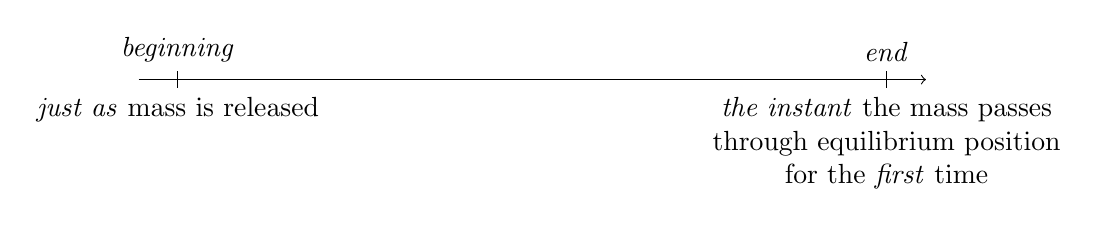
\begin{tikzpicture}
    % draw horizontal line   
    \draw[->] (0,0) -- (10,0);

    % draw vertical lines
    \foreach \x in {0.5,9.5}
      \draw (\x cm,3pt) -- (\x cm,-3pt);

    % draw nodes
    \draw (0.5,0) node[below=3pt] {\emph{just as} mass is released} node[above=3pt] {\emph{beginning}};
    \draw (9.5,0) node[below=3pt, align=center] {\emph{the instant} the mass passes\\through equilibrium position\\for the  \emph{first} time} node[above=3pt] {\emph{end}};
\end{tikzpicture}
\end{center}

\begin{enumerate}
	\item What {\em properties} of the physical system (indicators) changed significantly between the initial and final state?  What energy systems are associated with those indicators?
	\label{act212.2-3}
	
	\item Make a complete \EnergyDiagram{}:
	\label{act212.2-4}
		
	Show the increases and decreases in the energy systems and show the initial and final values of the indicator associated with each energy system -- be as explicit as possible.
	
	\item Write down an algebraic representation of your \EnergyDiagram, expressing energy conservation.

\end{enumerate}

\WCD  

\subsection{Reflecting on the \SOModel{}}

\begin{enumerate}
	\item Do changes in the energy systems you identified depend on the direction that the indicator changed (the sign of the indicator), or only on the magnitude of the indicator?
	
	\note{}{
	In other words, when is thermal energy significant? The model would be the same for the 2nd time through.  By the 20th we would expect the spring-mass to be slowing down.  In modeling the process they would need to include a third energy system�a thermal energy system (the way we take friction into account with our energy-interaction model).   Whether to take dissipation into account explicitly in developing any particular model, depends on whether it is significant.  Does it show up on your measurement instrument?  In this case, do we see it making a difference?  Same with rock and coffee filter.  If we see it, and it �bothers� us, we put it in.
	}
	\item Would the way you modeled this physical system be any different from what you did in your response to \hyperref[act212.2-4]{\ref*{act212.2}\#\ref*{act212.2-4}} if the \textbf{final state} were the instant the mass returned to its equilibrium position the second time, instead of the first?  How about if it were the 200th time?
\end{enumerate}

\note{}{
In the final \WC{} discussion you should ask students how what they did with mechanical energies was similar to what they did with internal energies and what is different, if anything?
}
\WCD